% ============================================================
% image5 —— 矩形 ABCD 沿对角线 AC 折起（B、D 分别向 AC 作垂线，垂足 M、N）
% 源位图：工作区/字替对照-0909/variantF/media/media/image5.png（1798×1350 px）
% 源排印宽 54.7mm ⇒ 1 px = 54.7/1798 = 0.0304227 mm（两轴同尺，源图无纵横压缩）
% 依赖：仅 tikz（\usetikzlibrary 都不用）
%
% 【线宽折算】源图实/虚一律 10px 粗 ⇒ line width = 10×0.0304227 = 0.3042mm（≈0.864pt）
% 【虚线折算】源图虚线节距实测：实 40px、空 20px ⇒ on 1.2169mm / off 0.6085mm（周期 1.8254mm）
%              （AC/BM/MD 实测周期 60px；DN 实测 62～63px，属栅格化误差，统一取 60px）
% 【字号折算】源图标签字冠高 110～115px（均 112px）。源图字形度量与 Times 斜体吻合
%             （Times 冠高 0.662em ⇒ em = 112/0.662 = 169px = 5.14mm = 14.6pt）。
%             本图沿用项目先例的西文数学斜体（cmmi，冠高 0.683em），CM 字号为定档
%             （10 / 12 / 14.4 / 17.28…），14.6pt 只能落 14.4pt；非定档字号会被 LaTeX
%             静默替代成最近档（实测 13.6pt→14.4pt），故径直声明 14.4pt：换任何宿主
%             都不产生字号替代告警，且与「源图折算 14.6pt」仅差 1.4%。
%             实测重绘标签冠高 114px vs 源 112px（+1.8%），字面宽 +1%～+14%（cmmi 的
%             A/B/C 比 Times 斜体宽，D/M/N 几乎等宽），见核对表 §三。
%
% 【坐标】x 正向＝源图右，y 正向＝源图上（source px → (px_x·s, (1350-px_y)·s)）
%   顶点   源图像素(中心线交点)      本文件坐标(mm)
%   A      ( 130.33 ,  737.79 )     ( 3.9650 , 18.6187 )   实线 AB、AD 交点
%   B      ( 647.41 ,  174.46 )     (19.7139 , 35.7637 )   B.x 取 BM 垂线 x=648px 对齐
%   C      (1658.04 ,  738.19 )     (50.4429 , 18.6187 )   C.y 取 AC 水平线 y=738px
%   D      (1246.83 , 1145.02 )     (37.9027 ,  6.2360 )   D.x 取 DN 垂线 x=1246px 对齐
%   M      ( 648.00 ,  738.00 )     (19.7139 , 18.6187 )   B 在 AC 上的垂足
%   N      (1246.00 ,  738.00 )     (37.9027 , 18.6187 )   D 在 AC 上的垂足
%   标签中心（各自字形墨迹外接框中心，mm）
%   A(1.5363,18.8164) B(19.6531,38.5101) C(53.1180,18.9686) D(37.8763,3.2552)
%   M(16.7477,21.8435) N(37.9219,21.0981)
%   注：源图 C 标签被画布右边界裁去右端约 7px（源图墨迹 x 至 1797 仍在延伸），
%       本文件按完整字形放置，故重绘右边界略超 54.7mm（见核对表 §偏差）。
%
% 【图元清单】实线：AB、BC、CD、DA、BD（BD＝折起后 B、D 连线）；虚线：AC、BM、DN、MD
%             无箭头、无向量符号、无直角标记、无辅助圆
% ============================================================
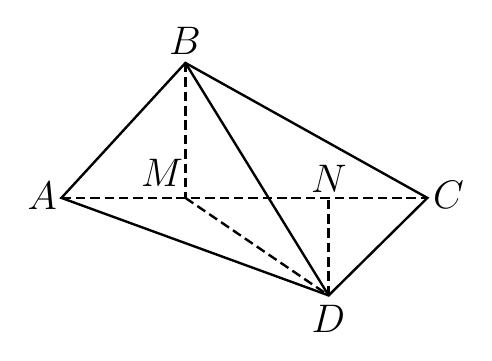
\begin{tikzpicture}[
  x=1mm, y=1mm,
  line width=0.3042mm,
  line cap=butt, line join=miter,
  im5dash/.style={dash pattern=on 1.2169mm off 0.6085mm},
  every node/.style={inner sep=0pt, font=\fontsize{14.4pt}{14.4pt}\selectfont}
]
  % ---- 顶点 ----
  \coordinate (A) at ( 3.9650,18.6187);
  \coordinate (B) at (19.7139,35.7637);
  \coordinate (C) at (50.4429,18.6187);
  \coordinate (D) at (37.9027, 6.2360);
  \coordinate (M) at (19.7139,18.6187);
  \coordinate (N) at (37.9027,18.6187);
  % ---- 实线：两个三角形的边 + 折起后 BD ----
  \draw (A) -- (B) -- (C) -- (D) -- cycle;
  \draw (B) -- (D);
  % ---- 虚线：对角线 AC、垂线 BM、垂线 DN、MD（源图 M–D 亦为虚线） ----
  \draw[im5dash] (A) -- (C);
  \draw[im5dash] (B) -- (M);
  \draw[im5dash] (D) -- (N);
  \draw[im5dash] (M) -- (D);
  % ---- 标签（西文斜体数学体，anchor=center 对准源图字形中心） ----
  \node at ( 1.5363,18.8164) {$A$};
  \node at (19.6531,38.5101) {$B$};
  \node at (53.1180,18.9686) {$C$};
  \node at (37.8763, 3.2552) {$D$};
  \node at (16.7477,21.8435) {$M$};
  \node at (37.9219,21.0981) {$N$};
\end{tikzpicture}
